%--------------------------------------------------------------------
% NE 155 (intro to numerical simulation of radiation transport)
% Spring 2014

% formatting
\documentclass[12pt]{article}
\usepackage[top=1in, bottom=1in, left=1in, right=1in]{geometry}

\usepackage{setspace}
\usepackage{tabu}
\onehalfspacing

\setlength{\parindent}{0mm} \setlength{\parskip}{1em}


% packages
\usepackage{amssymb}
%% The amsthm package provides extended theorem environments
\usepackage{amsthm}
\usepackage{epsfig}
\usepackage{times}
\renewcommand{\ttdefault}{cmtt}
\usepackage{amsmath}
\usepackage{graphicx} % for graphics files

% Draw figures yourself
\usepackage{tikz} 

% The float package HAS to load before hyperref
\usepackage{float} % for psuedocode formatting
\usepackage{xspace}

% from Denovo methods manual
\usepackage{mathrsfs}
\usepackage[mathcal]{euscript}
\usepackage{color}
\usepackage{array}

\usepackage[pdftex]{hyperref}

\newcommand{\nth}{n\ensuremath{^{\text{th}}} }
\newcommand{\ve}[1]{\ensuremath{\mathbf{#1}}}
\newcommand{\macro}{\ensuremath{\Sigma}}
\newcommand{\vOmega}{\ensuremath{\hat{\Omega}}}

\newcommand{\cc}[1]{\ensuremath{\overline{#1}}}
\newcommand{\ccm}[1]{\ensuremath{\overline{\mathbf{#1}}}}


%--------------------------------------------------------------------
%--------------------------------------------------------------------
\begin{document}
\begin{center}
{\bf NE 155, Midterm 2 Review S15}
\end{center}

The exam will be 50 minutes long and closed book. You may use a calculator and have a 1-page notes sheet (front and back) that you will turn in with the exam.

\setlength{\unitlength}{1in}
\begin{picture}(6,.1) 
\put(0,0) {\line(1,0){6.25}}         
\end{picture}

%--------------------------------------------------------------------
Here are the topics we've covered and that are fair game for the exam:

The exam will be 50 minutes long and closed book. \\
You may use a calculator.\\
You may have an 8.5" x 11" page with writing on \textbf{ONE} side. You must turn it in with the exam.

\section*{More deterministic methods}
Think about what things are reasonable to ask on a 50 minute exam when you can't solve anything with a computer: forms of equations, meaning, trends, etc.
\begin{itemize}
\item Iterative solutions of linear systems
  \begin{itemize}
  \item General form of the fixed point iterative method
  \item Richardson / Source interation
  \item Jacobi
  \item Gauss Seidel
  \item SOR
  \item convergence
  \item preconditioning
  \end{itemize}


\item Finite difference derivation; application to the 1-D, fixed source diffusion equation
\item Finite volume method (1-D and 2-D)
  \begin{itemize}
  \item Derivation
  \item Application to the diffusion equation
  \item Vacuum and reflecting boundary conditions
  \item Simplification to homogeneous, uniform mesh
  \end{itemize}
  
\item Methods for solving the system of equations we created
  \begin{itemize}
  \item Directly with Thomas Algorithm
  \item Iteratively with Jacobi, GS, or SOR
  \end{itemize}

\item Eigenvalue form of the DE
  \begin{itemize}
  \item form of the equation; applying finite difference
  \item applying finite volume method, including BCs
  \end{itemize}
  
\item Solving the Eigenvalue equations
  \begin{itemize}
  \item determining convergence of $k$ and $\phi$
  \item calculating $k$
  \item Power Iteration
  \end{itemize}
\end{itemize}

%-------------------------------------------------------------
\section*{Point Kinetics and Taylor/RK}
\begin{itemize}
\item What the point kinetics equation is, including terms and assumptions
\item Units of reactivity; what is reactor period 
\item Simple solutions of the PRKE
\item Taylor series and Runge Kutta are two methods for solving the PRKE
\end{itemize}


%-------------------------------------------------------------
\section*{MC: Math with Random Numbers}
You can use random numbers to do math in two primary ways: 
\begin{itemize}
\item sample physical distributions to reproduce physics needed to solve  problems
\item conduct numerical integration to solve problems
\end{itemize}

You would choose to do Monte Carlo when 
\begin{itemize}
\item analytical integration is impossible
\item deterministic methods are too slow, require approximations that don't work, you can't get the solution, etc.
\end{itemize} 

A good thing to think about is this comparison of methods
\begin{center}
\begin{tabu}{| l | X | X |}
  \hline
  & Monte Carlo         & Deterministic \\\hline
              % -----------------------
    Strengths & * General geometry    & * Fast \\
              & * Continuous Energy   & * Global Solution\\
              & * Continuous in Angle & * Solution is of same quality everywhere\\
              & * Inherently 3-D      & \\
              & * Easy to parallelize on CPUs & \\\hline
% -----------------------
    Weaknesses & * Slow & * Variable discretization governs solution quality \\
               & * Might be memory intensive & * Might be memory intensive \\
               & * Solutions have statistical error & * Solution contains truncation error\\
               & * Local solutions only & * Constrained by what you can mesh \\
               & * Must adequately sample phase space & * Ray Effects \\
               & * Need efficient VR & * Can be complicated to parallelize on CPUs \\\hline
  \end{tabu}
\end{center}


%-------------------------------------------------------------
\section*{MC algorithm}
\begin{figure}[h]
\begin{center}
  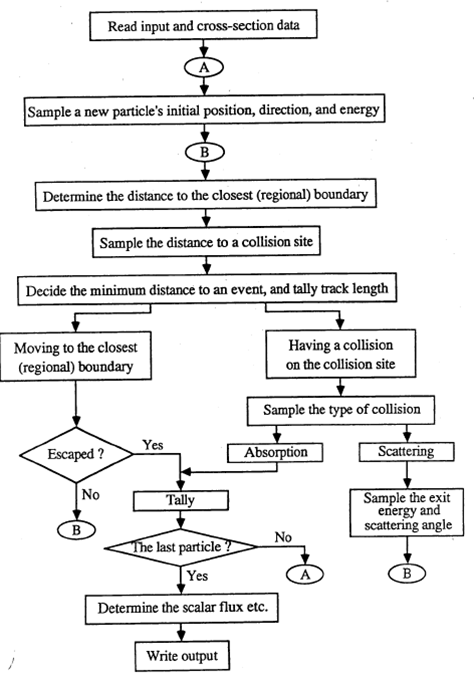
\includegraphics[height=6 in,clip]{monte-carlo/MC-algorithm}
  \caption{Monte Carlo neutral particle transport algorithm}
  \end{center}
  \label{fig:mc-algo}
\end{figure}

Figure 1 shows the algorithm that is basically what happens in MC. We learned the items needed to do all of these steps.


%--------------------------------------------------------
\subsection*{PDFs, CDFs}
We learned how to define PDFs and CDFs for continuous and discrete variables; including how to normalize them. 

%--------------------------------------------------------
\subsection*{Sampling}
We learned how to sample different kinds of CDFs. An example of direct inversion is determining the \textbf{distance to the next interaction} (we also did this as a function of mean free path only):

\begin{itemize}
\item $\Sigma_t$ = total macroscopic cross section of material
\[\Sigma_T = \sum_{j=1}^J N_j \sigma_t^j\]

\item The PDF for distance to collision is probability of interaction per unit distance $\times$ probability of traveling distance $s$ without interacting
\[g(s) = \Sigma_t \exp\bigl(-\Sigma_t s \bigr)\]

\item We integrate and normalize to get the CDF
\[G(s) = 1 - \exp\bigl(-\Sigma_t s \bigr)\]

\item To actually sample this, we invert it and get a random number
\[s = \frac{-\ln(\xi)}{\Sigma_t}\]
\end{itemize}
%
If we're in a multi-region problem, we figure out if we intersect a boundary and if so move the particle to that boundary and determine how much farther it goes into the next material before having a collision.

After finding the location of the collision and the isotope collided with, we need to determine \textbf{what type of collision} occurs. 

\begin{itemize}
\item $\Sigma_t = \Sigma_{elastic} + \Sigma_{inelastic} + \Sigma_{capture} + \Sigma_{fission} + \dots$.

\item The probability of reaction of type $i$ for a given isotope is 
\[p_i = \frac{\Sigma_i}{\Sigma_t}\]

\item This gives a set of discrete probabilities, which we can sample 
\begin{itemize}
\item directly: generate $\xi$, determine $k$ s.t. $G_{k-1} \leq \xi \le G_k$, return $i = i_k$.

\item or by making an alias table and sampling.
\end{itemize}

\end{itemize}


%--------------------------------------------------------
\subsection*{Tallies}

We also talked about how to get results through 
\begin{itemize}
\item \textbf{estimators}: convert each history into a score, that are summed together to create 
\item \textbf{tallies}: a set of scores that for a PDF whose expected value should converge to the solution of interest.
\end{itemize}

We talked about a variety of formulas for how to do this. 


%--------------------------------------------------------
\subsection*{Statistics}

Monte Carlo solution statistics are based on the Central Limit Theorem, which is applicable when samples are taken from the same distribution (identical) and they are independent of one another. 

In this case we can assert formulas for the sample mean, error, and variance and relate those to the true mean, error, and variance. 

We have the ability to measure precision and criteria for determining how precise an answer must be for it to be acceptable. 


\end{document}